% Options for packages loaded elsewhere
\PassOptionsToPackage{unicode,linktoc=all}{hyperref}
\PassOptionsToPackage{hyphens}{url}
\PassOptionsToPackage{dvipsnames,svgnames,x11names}{xcolor}
%
\documentclass[
  a4paper,
]{article}
\usepackage{amsmath,amssymb}
\usepackage{lmodern}
\usepackage{iftex}
\ifPDFTeX
  \usepackage[T1]{fontenc}
  \usepackage[utf8]{inputenc}
  \usepackage{textcomp} % provide euro and other symbols
\else % if luatex or xetex
  \usepackage{unicode-math}
  \defaultfontfeatures{Scale=MatchLowercase}
  \defaultfontfeatures[\rmfamily]{Ligatures=TeX,Scale=1}
\fi
% Use upquote if available, for straight quotes in verbatim environments
\IfFileExists{upquote.sty}{\usepackage{upquote}}{}
\IfFileExists{microtype.sty}{% use microtype if available
  \usepackage[]{microtype}
  \UseMicrotypeSet[protrusion]{basicmath} % disable protrusion for tt fonts
}{}
\makeatletter
\@ifundefined{KOMAClassName}{% if non-KOMA class
  \IfFileExists{parskip.sty}{%
    \usepackage{parskip}
  }{% else
    \setlength{\parindent}{0pt}
    \setlength{\parskip}{6pt plus 2pt minus 1pt}}
}{% if KOMA class
  \KOMAoptions{parskip=half}}
\makeatother
\usepackage{xcolor}
\IfFileExists{xurl.sty}{\usepackage{xurl}}{} % add URL line breaks if available
\IfFileExists{bookmark.sty}{\usepackage{bookmark}}{\usepackage{hyperref}}
\hypersetup{
  pdftitle={Asking Questions in English},
  pdfauthor={R (Chandra) Chandrasekhar},
  pdflang={en-GB},
  colorlinks=true,
  linkcolor={DarkOliveGreen},
  filecolor={Purple},
  citecolor={DarkKhaki},
  urlcolor={Maroon},
  pdfcreator={LaTeX via pandoc}}
\urlstyle{same} % disable monospaced font for URLs
\usepackage[margin=25mm]{geometry}
\usepackage{longtable,booktabs,array}
\usepackage{calc} % for calculating minipage widths
% Correct order of tables after \paragraph or \subparagraph
\usepackage{etoolbox}
\makeatletter
\patchcmd\longtable{\par}{\if@noskipsec\mbox{}\fi\par}{}{}
\makeatother
% Allow footnotes in longtable head/foot
\IfFileExists{footnotehyper.sty}{\usepackage{footnotehyper}}{\usepackage{footnote}}
\makesavenoteenv{longtable}
\usepackage{graphicx}
\makeatletter
\def\maxwidth{\ifdim\Gin@nat@width>\linewidth\linewidth\else\Gin@nat@width\fi}
\def\maxheight{\ifdim\Gin@nat@height>\textheight\textheight\else\Gin@nat@height\fi}
\makeatother
% Scale images if necessary, so that they will not overflow the page
% margins by default, and it is still possible to overwrite the defaults
% using explicit options in \includegraphics[width, height, ...]{}
\setkeys{Gin}{width=\maxwidth,height=\maxheight,keepaspectratio}
% Set default figure placement to htbp
\makeatletter
\def\fps@figure{htbp}
\makeatother
\setlength{\emergencystretch}{3em} % prevent overfull lines
\providecommand{\tightlist}{%
  \setlength{\itemsep}{0pt}\setlength{\parskip}{0pt}}
\setcounter{secnumdepth}{-\maxdimen} % remove section numbering
\ifLuaTeX
\usepackage[bidi=basic]{babel}
\else
\usepackage[bidi=default]{babel}
\fi
\babelprovide[main,import]{british}
% get rid of language-specific shorthands (see #6817):
\let\LanguageShortHands\languageshorthands
\def\languageshorthands#1{}
% $HOME/.pandoc/defaults/latex-header-includes.tex
% Common header includes for both lualatex and xelatex engines.
%
% Preliminaries
%
\PassOptionsToPackage{rgb,dvipsnames,svgnames}{xcolor}
\PassOptionsToPackage{main=british}{babel}
\AtBeginEnvironment{quote}{\small}
\AtBeginEnvironment{quotation}{\small}
\AtBeginEnvironment{longtable}{\centering}
%
% Packages that are useful to include
%
\usepackage{graphicx}
\usepackage{subcaption}
\usepackage[inkscapeversion=1]{svg}
\usepackage[defaultlines=4,all]{nowidow}
\usepackage[capitalize,noabbrev]{cleveref}
\usepackage{etoolbox}
\usepackage{fontsize}
\usepackage{newunicodechar}
\usepackage{pdflscape}
\usepackage{fnpct}
\usepackage{parskip}
  \setlength{\parindent}{0pt}
\usepackage[style=american]{csquotes}
% \usepackage{setspace} Use the <fontname-plus.tex> files for setspace
%
% $HOME/.pandoc/defaults/latex-header-includes.tex
% Common header includes for both lualatex and xelatex engines.
%
% Preliminaries
%
\PassOptionsToPackage{rgb,dvipsnames,svgnames}{xcolor}
\PassOptionsToPackage{main=british}{babel}
\AtBeginEnvironment{quote}{\small}
\AtBeginEnvironment{quotation}{\small}
\AtBeginEnvironment{longtable}{\centering}
%
% Packages that are useful to include
%
\usepackage{graphicx}
\usepackage{subcaption}
\usepackage[inkscapeversion=1]{svg}
\usepackage[defaultlines=4,all]{nowidow}
\usepackage[capitalize,noabbrev]{cleveref}
\usepackage{etoolbox}
\usepackage{fontsize}
\usepackage{newunicodechar}
\usepackage{pdflscape}
\usepackage{fnpct}
\usepackage{parskip}
  \setlength{\parindent}{0pt}
\usepackage[style=american]{csquotes}
% \usepackage{setspace} Use the <fontname-plus.tex> files for setspace
%
% charis-plus.tex
% Font-setting header file for use with Pandoc Markdown
% to generate PDF via LuaLaTeX.
% The main font is Charis SIL.
% Other main fonts are also available in appropriately named file.
\usepackage{fontspec}
\usepackage{setspace}
\setstretch{1.3}
%
\defaultfontfeatures{Ligatures=TeX,Scale=MatchLowercase,Renderer=HarfBuzz} % at the start always
%
% For English
%
\babelfont{rm}[Scale=1]{Merriweather}
\babelfont{sf}[BoldFont={* Semibold}]{Source Sans Pro}
\babelfont{tt}[Scale=0.9]{Fira Mono}
%
\babelprovide[import,onchar=ids fonts]{sanskrit}
\babelprovide[import,onchar=ids fonts]{tamil}
\babelprovide[import,onchar=ids fonts]{greek}
%
\babelfont[sanskrit]{rm}[Scale=1.1,Renderer=HarfBuzz]{Noto Serif Devanagari}
\babelfont[sanskrit]{sf}[Scale=1.1,Renderer=HarfBuzz]{Noto Sans Devanagari}
\babelfont[tamil]{rm}[Renderer=HarfBuzz]{Noto Serif Tamil}
\babelfont[tamil]{sf}[Renderer=HarfBuzz]{Noto Sans Tamil}
\babelfont[greek]{rm}{Gentium Book Plus}
%
% Math font
%
\usepackage{unicode-math} % seems not to hurt % fallabck
\setmathfont[bold-style=TeX]{STIX Two Math}
%
% Other fonts
%
\newfontfamily{\emojifont}{Symbola}
%
% indic-greekfonts.tex
% $HOME/.pandoc/defaults/indic-greek-fonts.tex
% $Usage: --include-in-header="$HOME/.pandoc/defaults/indic-greek-fonts.tex"
% Assumes that we already have
%
% \usepackage[main=british]{babel}
%
% in another header-includes file; % in this case
% "$HOME/.pandoc/defaults/latex-header-includes.tex"
%
% We use this file only when we need Tamil, Devanagari, Greek scripts.
% Do not invoke if not needed, to speed up compilation.
%
% Tamil, Devanagari, and Greek fonts
%
\newfontfamily\devanagarifont{Noto Serif Devanagari}
\newfontfamily\tamilfont{Noto Serif Tamil}
\newfontfamily\greekfont{Noto Serif}
%
% Put babel to work
%
\babelprovide[import onchar=ids fonts]{sanskrit}
\babelprovide[import onchar=ids fonts]{tamil}
\babelprovide[import onchar=ids fonts]{greek}
%
% Relative font sizes may be tweaked here for visual congruity
%
\babelfont[sanskrit]{rm}[Scale=1]{Noto Serif Devanagari}
\babelfont[sanskrit]{sf}[Scale=1]{Noto Sans Devanagari}
\babelfont[tamil]{rm}[Scale=0.9]{Noto Serif Tamil} % visual scaling to match
\babelfont[tamil]{sf}[Scale=0.9]{Noto Sans Tamil}
\babelfont[greek]{rm}[Scale=0.9]{Noto Serif}
\babelfont[greek]{sf}[Scale=0.9]{Noto Sans}
%
% NOTES
% Specific invocations when using lualatex as the engine.
% Especially useful with multi-lingual typesetting with babel.

% NOTE: xelatex works with polyglossia and ucharclasses; lualatex does not.
% Moreover, the package `ucharclasses` does not reliably preserve italics, etc.,
% when used in a mutli-script/multi-language setting.
%
% Accordingly, with multi-lingual documents, we should prefer
% lualatex with babel instead of xelatex with ucharclasses.
%
% See
% https://tex.stackexchange.com/questions/199773/how-to-type-hindi-words-in-latex/
%
% and
%
% https://tex.stackexchange.com/questions/613999/switching-between-three-scripts-using-ucharclasses-does-not-seem-to-work
%
% Use babel; since babel is in rapid development,
% this part could change in future.
%
%  Note that Sanskrit can have many scripts; we use Devanagari.
% This might need to be tweaked in future.
\usepackage{titling}
\usepackage{fancyhdr}
    \pagestyle{fancy}
    \fancyhead{}
    \fancyfoot{}
    \renewcommand{\headrulewidth}{0.2pt}
    \renewcommand{\footrulewidth}{0.2pt}
    \fancyhead[LO,RE]{\scshape\thetitle}
    \fancyfoot[CO,CE]{\footnotesize Copyright © 2006\textendash\the\year, R (Chandra) Chandrasekhar}
    \fancyfoot[RE,RO]{\thepage}
\usepackage{tcolorbox}
\usepackage{alltt}
\definecolor{noun}{HTML}{51847F}
\definecolor{pronoun}{HTML}{F0DFAB}
\definecolor{action}{HTML}{DCA3A3}
\definecolor{normal}{HTML}{DBDBDB}
\definecolor{background}{HTML}{363636}
\newcommand\noun[1]{\textcolor{noun}{#1}}
\newcommand\pronoun[1]{\textcolor{pronoun}{#1}}
\newcommand\action[1]{\textcolor{action}{#1}}
\newcommand\normal[1]{\textcolor{other}{#1}}
  \tcbset{boxrule=0mm, arc=0mm, colback=background}
\ifLuaTeX
  \usepackage{selnolig}  % disable illegal ligatures
\fi

\title{Asking Questions in English}
\author{R (Chandra) Chandrasekhar}
\date{2012-09-15 | 2022-05-29}

\begin{document}
\maketitle




\hypertarget{a-tale-of-two-tongues}{%
\subsection{A tale of two tongues}\label{a-tale-of-two-tongues}}

This blog is devoted to the art of asking questions correctly in
English. This seemingly undemanding task often trips up the aspiring
learner of English, especially one who is studying it as a second or
third language.

My mother tongue is
\href{http://en.wikipedia.org/wiki/Tamil_language}{Tamil,} written தமிழ்
(tamiḻ)\footnote{The transliteration adopted here follows
  \href{https://en.wikipedia.org/wiki/ISO_15919}{ISO 15919}}, in its
markedly curly script.\footnote{If you see rectangular boxes where you
  would expect to see letters, please ensure that you have a font on
  your device capable of displaying Tamil script.} Tamil is an
alphabetic, syllabic, inflected Indic language with ancient roots.
Asking questions in Tamil and English require two very different ways of
thinking and speaking. Knowing about these can be instructive to many
non-native speakers of English. Let me elaborate.

\hypertarget{word-order-in-english-and-tamil}{%
\subsection{Word order in English and
Tamil}\label{word-order-in-english-and-tamil}}

A friend, fairly proficient in English, but not so much in Tamil,
translated the question ``Can I come to your house now?'' into the Tamil
``முடியுமா நான் வருவதற்கு உங்கள் வீட்டுக்கு இப்பொழுது?'' (muḍiyumā nān
varuvadaṟku uṅgaḷ vīṭṭukku ippoḻudu?). This sentence replicates the
English word sequence faithfully, and while certainly not the best of
Tamil in elegance or usage, it is at least intelligible \emph{and}
grammatical. That is because Tamil is more of an
\href{http://en.wikipedia.org/wiki/Inflection}{inflected} language than
English, and is therefore less sensitive to change in meaning due to
change in word order.

But the reverse translation from Tamil into English, especially when
applied to asking questions, is infelicitous. Following Tamil word order
to phrase English questions often leads to ungrammatical and discordant
results. Let me give you some examples.

\hypertarget{where-are-you-going}{%
\subsubsection{``Where are you going?''}\label{where-are-you-going}}

Suppose you see someone and want to ask in Tamil where that person was
going. You would ask, in the less respectful mode of address used
between equals, ``நீ எங்கே போகிறாய்?'' (nī engē pōgiṟāi?). Translated
into English, these words literally become ``You where going?'' and that
is often how a newcomer to English, with a Tamil language background,
will at first speak.

\hypertarget{are-you-well}{%
\subsubsection{``Are you well?''}\label{are-you-well}}

When meeting someone, it is polite and customary to ask ``How are you?''
in English. In Tamil, the more sanguine ``நீங்கள் நலமா?'' (nīṅkaḷ
nalamā?) is used, where the respectful plural form of the second person
pronoun is employed. Literally, it is a statement, posed as a question,
with a slight raise in pitch at the end to indicate the interrogative
sense when spoken. And the \emph{literal} translation into English is
the strange-sounding ``You are well?'' instead of the correct ``Are you
well?''.

\begin{figure}
\hypertarget{fig:questions}{%
\centering
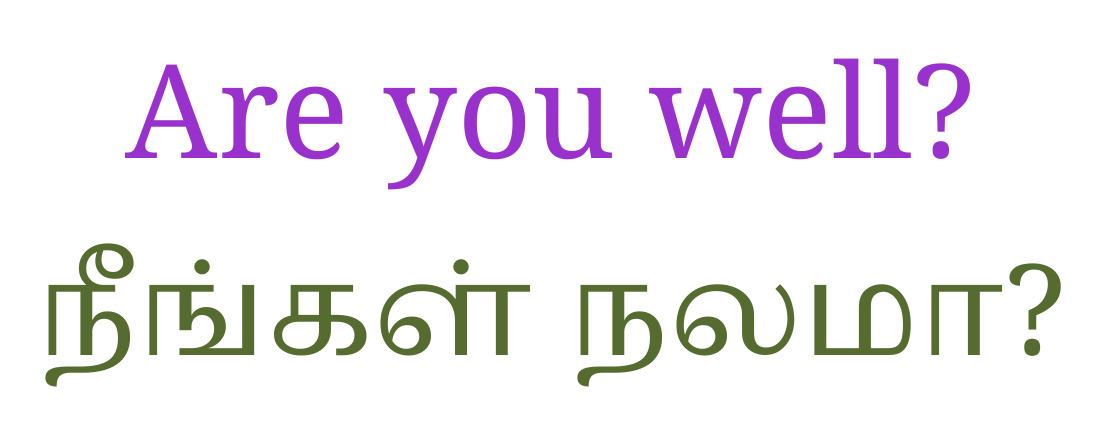
\includegraphics[width=0.8\textwidth,height=\textheight]{images/engtam.jpg}
\caption{The same question in English and Tamil; the latter version
\emph{literally} reads ``You are well?''.}\label{fig:questions}
}
\end{figure}

\hypertarget{what-is-your-name}{%
\subsubsection{``What is your name?''}\label{what-is-your-name}}

Now, for another example. When asking someone for his or her name, a
Tamil speaker says ``உன் பெயர் என்ன?'' (un peyar enna?). In English,
this word order would be rendered as ``Your name what?'' Horror of
horrors! Where has the verb gone?

\hypertarget{implicit-verbs-and-nouns}{%
\subsection{Implicit verbs and nouns}\label{implicit-verbs-and-nouns}}

We have all been taught that a complete sentence must have a verb. The
simplest sentence is an imperative ``Come!''. So, how did the Tamil
sentence dispense with the verb?

The Tamil speaker can likewise ask, ``Where is the subject in the
sentence `Come!'?''.

The answer to both questions is that usage has tacitly approved the
omission of the verb on the one hand, and the noun on the other. They
have become
\href{https://www.thefreedictionary.com/implicit}{\emph{implicit}}.

In Tamil, it is customary to omit the verb ``to be'' in its various
forms. Likewise, in English, the second person nominative singular
pronoun ``You''\footnote{Originally, this was ``Thou'' but the plural
  form ``You'' has supplanted it now.} has been omitted from the start
of the sentence ``Come!'' and its inclusion, rather than omission, will
raise eyebrows.

\hypertarget{word-order-in-english}{%
\subsection{Word order in English}\label{word-order-in-english}}

Because it is a less inflected language, word order matters more in
English than in Tamil. \emph{And word order is different for questions
in the two languages}. You should try to think in English before asking
a question in English. And likewise for Tamil.

Ancient languages tend to be inflected. Latin---once the bastion of
scholarly knowledge in Europe---is inflected. So too is Sanskrit which
served a similar historical role for the sacred and secular literature
of India. Ditto for Tamil, which of the three, is the only language that
is still widely spoken---by about 70 million people.

Unlike the more ancient tongues, English is less inflected. \emph{Word
order matters.} Meaning can and does change if word order is changed.
And many common mistakes in word order convey unintended humour or
absurdity.

The Latin sentence ``Amor vincit omnia'' meaning ``Love conquers all''
does not become ``All conquers love'' (whatever that may mean) if
rewritten as ``Omnia vincit amor''; it still carries the same meaning as
before.

English, however, is not immune to change of meaning with change of word
order. ``The cat ate the rat'' is believable, whereas, ``The rat ate the
cat'' is both unusual and incredible. Although I can see an enormous rat
polishing off a cat in my mind's eye, logic and experience tell me that
it is unlikely and runs against the grain of Nature.

Wrong word order in English, especially in questions, grates on the
ears. But before we progress to questions, we must peek at sentence
types and delve, however lightly, into some grammar.

\hypertarget{parts-of-speech-in-english}{%
\subsection{Parts of speech in
English}\label{parts-of-speech-in-english}}

I profess to be neither a grammarian nor a linguist. And both fields are
alive and growing. Take what I say below with this disclaimer in mind.

When I was taught English grammar, we were told that there were
\href{http://www.butte.edu/departments/cas/tipsheets/grammar/parts_of_speech.html}{eight
parts of speech}:

\begin{enumerate}
\tightlist
\item
  Noun
\item
  Pronoun
\item
  Verb
\item
  Adjective
\item
  Adverb
\item
  Preposition
\item
  Conjunction
\item
  Interjection
\end{enumerate}

The infusion of modern linguistics into English grammar has led to new
superclasses in parts of speech. An
\href{https://glossary.sil.org/term/adposition}{adposition} is a word
that can be either a \emph{preposition} or a \emph{postposition}.

Likewise, while we were taught about the indefinite articles \emph{a}
and \emph{an} and the definite article \emph{the}, these are nowadays
classified, along with a host of other miscellaneous language fragments,
as part of the superset called
\href{https://en.wikipedia.org/wiki/Determiner}{determiners}\footnote{Visit
  the website of
  \href{https://www.stthomaswernethprimary.co.uk/determiners-and-prepositions-1/}{St
  Thomas C of E Primary School} to watch and listen to two delightful
  videos on determiners and prepositions, if you feel so inclined.}.

Because our primary focus is on questions and word order in correctly
phrased questions, I will use the term
\href{https://en.wikipedia.org/wiki/Interrogative_word}{\emph{interrogative}}
to apply to any word, like \emph{what}, which signals a question in
English. Such interrogatives could actually be functioning as pronouns,
adverbs, adjectives, etc., depending on their place and meaning in a
sentence.

\hypertarget{sentence-types}{%
\subsection{Sentence types}\label{sentence-types}}

Classic textbooks on English grammar identify \emph{four} kinds of
sentences:

\begin{enumerate}
\item
  Declarative: ``Today is Thursday.'' These types of sentences simply
  state facts. They are also called statements or assertions.
\item
  Interrogative: ``What is your name? Sentences of this type are
  questions.
\item
  Imperative: ``Come here.'' This is a command \footnote{ As we have
    already seen, the \emph{implicit subject} of this sentence is the
    pronoun ``You'' which should rightly have come first, so that the
    sentence reads ``You come here.'' Leaving out the understood second
    person pronoun has become established usage; so we omit it.}.
\item
  Exclamatory: ``How nice!'' This type of sentence carries strong
  emotional overtones which distinguish it from a plain assertion.
\end{enumerate}

Suppose, I said ``Thank you!'' with all sincerity and gratitude, that
would also count as an exclamatory sentence.

But wait a moment: who or what is the subject here? We encounter the
implicit subject once again: only here it is the first person nominative
singular pronoun ``I''. So, the sentence should rightfully read ``I
thank you!'' but it would be hard to exclaim it convincingly without
sounding theatrical.

The addition of the pronoun ``I'' thus converts the sentence from an
exclamatory into a declarative one (work out why, and whether the
exclamation mark is appropriate).

Although grammarians recognize four sentence types, we have already seen
from the last example that an exclamatory sentence may be transformed
with ease into a declarative sentence simply by including an omitted
pronoun. Perhaps there are only three sentence types.

In one sense, all such classifications are artificial analytical
superimpositions on the body of a living language. Hence, it is more
important to master the language and its usage than to parrot out
classifications like the above.

\hypertarget{statements-versus-questions}{%
\subsection{Statements versus
Questions}\label{statements-versus-questions}}

It is important, however, to distinguish between a statement and a
question. They are two very different types of sentence, almost
antithetical in nature. Their word order is accordingly different:
something that is not often grasped by speakers whose first language is
not English.

A \emph{statement} in English usually has the abstract structure:

\begin{tcolorbox}
\begin{alltt}
\color{normal}
[\noun{Noun}/\pronoun{Pronoun}] [\action{Verb}] [\noun{Noun}/\pronoun{Pronoun}]
\end{alltt}
\end{tcolorbox}

where the first noun/pronoun is the \emph{subject} and the second
noun/pronoun, if it exists, is the \emph{object.} An example is ``He
kicked the ball''. This is in \emph{active voice.} In \emph{passive
voice} though, we say, ``The ball was kicked by him'', and the order of
the nouns/pronouns is changed.

A \emph{question} on the other hand has a different structure:

\begin{tcolorbox}
\begin{alltt}
\color{normal}
[Interrogative] [\action{Verb}] [\noun{Noun}/\pronoun{Pronoun}]
\end{alltt}
\end{tcolorbox}

The \emph{interrogative} is a word like ``what'' or ``why'' or ``where''
or ``how'' which is used to indicate that a question is being asked.
Having it at the beginning is handy because it alerts the listener to
the fact that a question is being asked, for which an answer would most
likely be required in response.

Note carefully that the verb comes \emph{before} the subject which is
the noun/pronoun at the end\footnote{If you consider the noun/pronoun at
  the end as the object, feel free to do so. We are talking correct
  usage here rather than grammar.}.

\hypertarget{inversion-of-a-statement-into-a-question}{%
\subsection{Inversion of a statement into a
question}\label{inversion-of-a-statement-into-a-question}}

A statement and a question are therefore different in structure. Many
speakers learning English invert a statement into a question by simply
raising the pitch at the end. So, they say ``You are well?'' raising the
pitch of the last word instead of asking ``Are you well?''. This is
wrong, although it happens a great deal in casual conversation. It will
never do for written English. To avoid falling into this trap, think:

\begin{tcolorbox}
\begin{alltt}
\color{normal}
Statement → [\noun{Noun}/\pronoun{Pronoun}] before [\action{Verb}]
Question  → [\action{Verb}] before [\noun{Noun}/\pronoun{Pronoun}]
\end{alltt}
\end{tcolorbox}

\hypertarget{a-very-simple-first-question}{%
\subsection{A very simple first
question}\label{a-very-simple-first-question}}

The simplest question in English is something like ``How are you?'' or
``What is this?''. Each consists of three words and the word order is
\texttt{{[}Interrogative{]}\ {[}Verb{]}\ {[}Noun/Pronoun{]}} exactly as
in our paradigm above.

\hypertarget{a-second-less-simple-question}{%
\subsection{A second less simple
question}\label{a-second-less-simple-question}}

The question ``What is your name?'' follows the above pattern too, but
it is complicated by the word ``your''. What does it do? It
\emph{qualifies} the noun ``name'' and is therefore an
adjective\footnote{Also called a \emph{possessive determiner} in modern
  grammatical usage.}. In English the adjective \emph{precedes} or comes
\emph{before} the noun.\footnote{In
  \href{http://en.wikipedia.org/wiki/Bahasa_Malaysia}{Bahasa Malaysia},
  the adjective \emph{succeeds} or \emph{comes after} the noun that it
  qualifies. Languages vary as do people.} This word order is not
altered in questions. Analytically, we may say:

\begin{longtable}[]{@{}ll@{}}
\toprule
Word & Part of Speech \\
\midrule
\endhead
What & interrogative (strictly interrogative pronoun) \\
is & verb \\
your & adjective; possessive case of pronoun ``you''; qualifies noun
``name'' \\
name & noun \\
\bottomrule
\end{longtable}

\hypertarget{mangled-questions}{%
\subsection{Mangled questions}\label{mangled-questions}}

When the word order in a properly constituted English question is
changed, it becomes what I call a \emph{mangled question.} Let us start
off with our last example and jumble it up to yield different mangled
questions.

\hypertarget{what-is-your-name-1}{%
\subsubsection{``What is your name?''}\label{what-is-your-name-1}}

With four unique words, we have a total of
\(4 \times 3 \times 2 \times 1 = 24\) different possible word orders and
thus sentences.

Rather than crunch our mind-numbing way through them all, let us look at
some more promising entries for the ``mangled question competition''. We
will use one guiding principle. The adjective ``your'' will always come
\emph{before} ``name'' \emph{if it appears at all} in the mangled
question.

\begin{tcolorbox}
\begin{alltt}
\color{normal}
What \noun{name}?
What \pronoun{your} \noun{name}?
What \pronoun{your} \noun{name} \action{is}?
What \action{is} \pronoun{your} \noun{name}?
\noun{Name} what?
\noun{Name} \action{is} what?
\noun{Name} what \action{is}?
\pronoun{Your} \noun{name} what?
\pronoun{Your} \noun{name} \action{is} what?
\pronoun{Your} \noun{name} what \action{is}?
\end{alltt}
\end{tcolorbox}

By now you should have got the drift. Once the interrogative has been
migrated to the beginning of the sentence and the verb placed to
immediately follow it, we have left as possibilities only:

\begin{enumerate}
\def\labelenumi{\alph{enumi}.}
\tightlist
\item
  the correct ``What is your name?''; and
\item
  the patently absurd ``What is name your?'' which we have already
  excluded from consideration.
\end{enumerate}

Voila!

\hypertarget{where-are-you-going-1}{%
\subsubsection{``Where are you going?''}\label{where-are-you-going-1}}

The second question, ``Where are you going?'' offers more scope for
creative misplacement of the verb because the verb itself consists of
two words rather than one, indicating the present continuous tense.

Again, I will not agonize over all 24 possibilities but will once more
restrict myself to ``promising mangled questions''. Almost instinctively
we will shirk from ever using that word-pair ``going are'' whereas the
alternative ``are going'', whole or split, is featured in full glory in
our entries to the mangled question contest.

\begin{tcolorbox}
\begin{alltt}
\color{normal}
\pronoun{You} where \action{going}?
\pronoun{You} where \action{are going}?
\pronoun{You} \action{going} where?
\pronoun{You} \action{are} where \action{going}?
\pronoun{You} \action{are going} where?
\action{Are going} where?
\action{Are} \pronoun{you} \action{going} where?
\action{Are going} where \pronoun{you}?
Where \action{going}?
Where \action{are going}?
Where \action{are going} \pronoun{you}?
Where \pronoun{you} \action{are going}?
Where \action{are} \pronoun{you} \action{going}?
\action{Going} where?
\action{Going} where \pronoun{you}?
\end{alltt}
\end{tcolorbox}

Choosing the correct version, though, is not as open and shut as before.
The strict but mindless application of the question paradigm
\texttt{{[}Interrogative{]}\ {[}Verb{]}\ {[}Noun/Pronoun{]}} to the
present continuous verb word-pair ``are going'' will lead to the mangled
sentence ``Where are going you?''.

In the correct version, ``Where are you going?'', we have the pronoun
juxtaposed between the two parts of the verb word-pair as ``are you
going''. It appears that the abstract structure for a question needs to
be modified somewhat.

\hypertarget{a-more-complicated-question}{%
\subsection{A more complicated
question}\label{a-more-complicated-question}}

In the previous example, the verb was in two parts as ``are going'' and
the noun was placed between them, which is easy enough. But English
verbs may have three parts as well, in the perfect tenses. Where would
we then put the noun or pronoun?

One easy way to work toward a solution is to \emph{start with a
statement and then convert it to a question}. Try this always when you
are stuck.

Suppose the statement is ``He has been recognized with a medal.'' One
could frame many questions from this one statement. Here are a few
grammatically correct examples:

\begin{tcolorbox}
\begin{alltt}
\color{normal}
\action{Has} \pronoun{he} \action{been recognized}?
How \action{has} \pronoun{he} \action{been recognized}?
Why \action{has} \pronoun{he} \action{been recognized}?
With what \action{has} \pronoun{he} \action{been recognized}?
\end{alltt}
\end{tcolorbox}

Note the following points:

\begin{itemize}
\item
  The first question has no interrogative as the first word, but rather
  starts off with the verb. Nevertheless it is a properly formed
  question. Here we have to grapple with the placement of the pronoun
  ``he'' within the triple-barrelled verb. The correct placement, shown
  here, applies to all the questions.
\item
  The second question might lay legitimate claim to being the closest in
  sense to an inversion of the original statement, ``He has been
  recognized with a medal.''.
\item
  The third and fourth questions are allied to the statement but are not
  really inversions of the original statement into a question. Their
  foci are different.
\end{itemize}

Suppose for a moment that we did not know where to place the pronoun
within the verb-triple. We know that the pronoun must be preceded by one
or more members of a verb-triple. We have only three choices:

\begin{tcolorbox}
\begin{alltt}
\color{normal}
How \action{has} \pronoun{he} \action{been recognized}?
How \action{has been} \pronoun{he} \action{recognized}?
How \action{has been recognized} \pronoun{he}?
\end{alltt}
\end{tcolorbox}

Of these, only the first is correct as deemed by usage. Again, if you
are attuned to usage, you would pick the first and reject the other two,
as easily as you would detect and discard two bad eggs out of a clutch
of three. Where to split the verb and insert the noun becomes an art
that you acquire with increasing facility in and exposure to English.
Familiarity with usage is more important than rule-based knowledge of
grammar.

The two lessons from this example are that:

\begin{enumerate}
\item
  A question \emph{can} begin without an interrogative.
\item
  The verb comes first followed by the noun/pronoun succeeded by the
  rest of the verb if applicable.
\end{enumerate}

\hypertarget{usage-changes}{%
\subsection{Usage changes}\label{usage-changes}}

Usage changes in verb tenses, and their quirks, pose yet another burden
to the student of English, especially when framing questions. Consider
the statement ``He ran fast.'' To invert it to a question, we may ask,
``How did he run?''.

Now, where was the ``did'' in the original statement? We could have
correctly said ``He \emph{did} run fast,'' but that would sound either
archaic or convey a specific emphatic sense, as if to refute a statement
that he did not run fast, or to emphasize that he ran very fast. But
these are different from the bland but neutral statement, ``He ran
fast,'' that we started out with.

If ``He ran fast,'' is all we have, simple application of the structure
we have derived would give us the question ``How ran he?'' which,
although correct, sounds decidedly poetic or archaic. Such expressions
are not in contemporary use.

Heaven forbid, if we said, ``How did he \emph{ran}?'' We would then be
committing a grammatical offense common to learners of English. Perhaps
the only way to avoid such errors is to listen, read, write, and speak,
until we become inwardly attuned to the language.

So, splitting a verb to insert a noun or pronoun to generate a question
is not simply a matter of rules but also of usage. By exposure to
correct spoken and written English, you should develop your own inner
sense of what is right and wrong. Rules, although helpful, are not a
reliable rescue when faced with changing patterns of usage.

\hypertarget{closing-comments}{%
\subsection{Closing comments}\label{closing-comments}}

English usage is variable and not wholly rule-bound. The large variety
of ways in which questions may be phrased precludes a simple abstract
formulation for the structure of a question along the lines of the
\href{http://en.wikipedia.org/wiki/Backus_Naur_form}{Backus-Naur form}
for the syntax of computer languages.

The facts we have here divined so far are:

\begin{enumerate}
\item
  The interrogative, if it exists, comes first.
\item
  The whole or part of the verb comes next.
\item
  The noun or pronoun follows.
\item
  The rest of the verb, if applicable, follows the noun or pronoun.
\item
  Adjectives and adverbs keep their relative word order.
\end{enumerate}

The abstract structure of a question, taken more as a flexible guide
than a rule cast in stone, is:

\begin{tcolorbox}
\begin{alltt}
\color{normal}
[Optional Interrogative] [\action{First part of Verb}] [\noun{Noun}/\pronoun{Pronoun}] [\action{Rest of \newline Verb if applicable}]
\end{alltt}
\end{tcolorbox}

Hopefully, this blog will help ensure that when you ask questions in
English you neither embarrass yourself by wrong or inelegant usage nor
confuse your interlocutor with a mangled question.

Happy questioning! \emojifont {🙂} \normalfont

\hypertarget{feedback}{%
\subsection{Feedback}\label{feedback}}

Please \href{mailto:feedback.swanlotus@gmail.com}{email me} your
comments and corrections.

\noindent A PDF version of this article is
\href{./asking-questions-in-english.pdf}{available for download here}:

\begin{normalsize}

\begin{ttfamily}

\url{https://swanlotus.netlify.app/blogs/asking-questions-in-english.pdf}

\end{ttfamily}

\end{normalsize}



\end{document}
